\begin{figure}
    \centering
    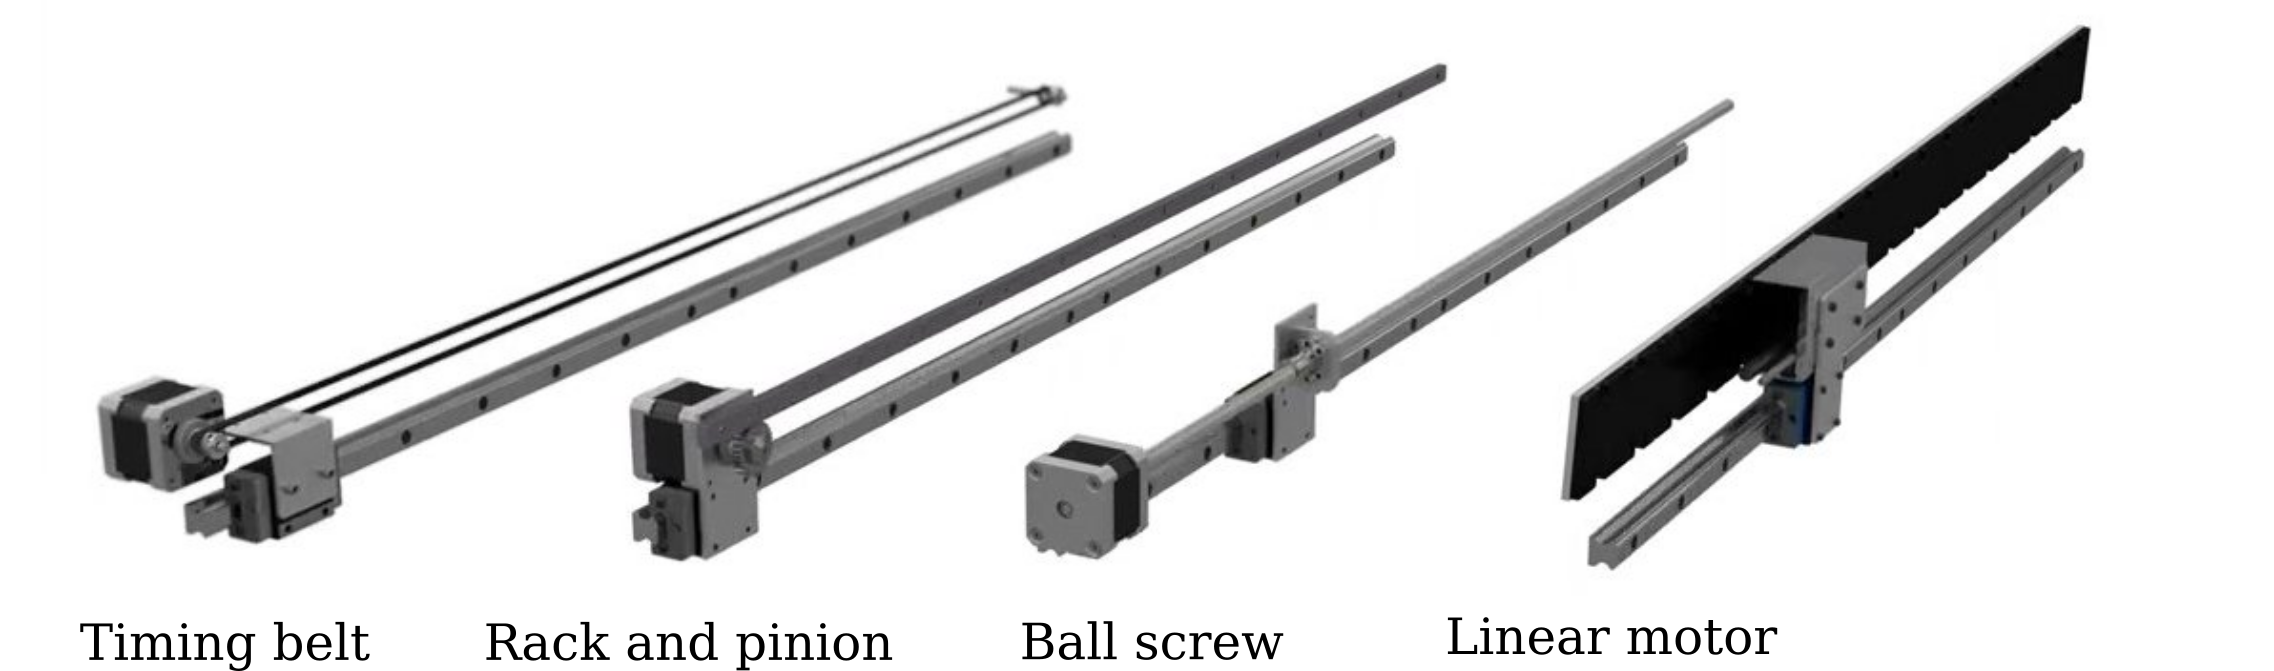
\includegraphics[width=0.9\textwidth]{linear-motion-systems}
    \caption{Linear motion systems}
    \label{fig:linear-motion-systems}
\end{figure}

\begin{figure}
    \centering
    \begin{subfigure}[b]{0.4\textwidth}
        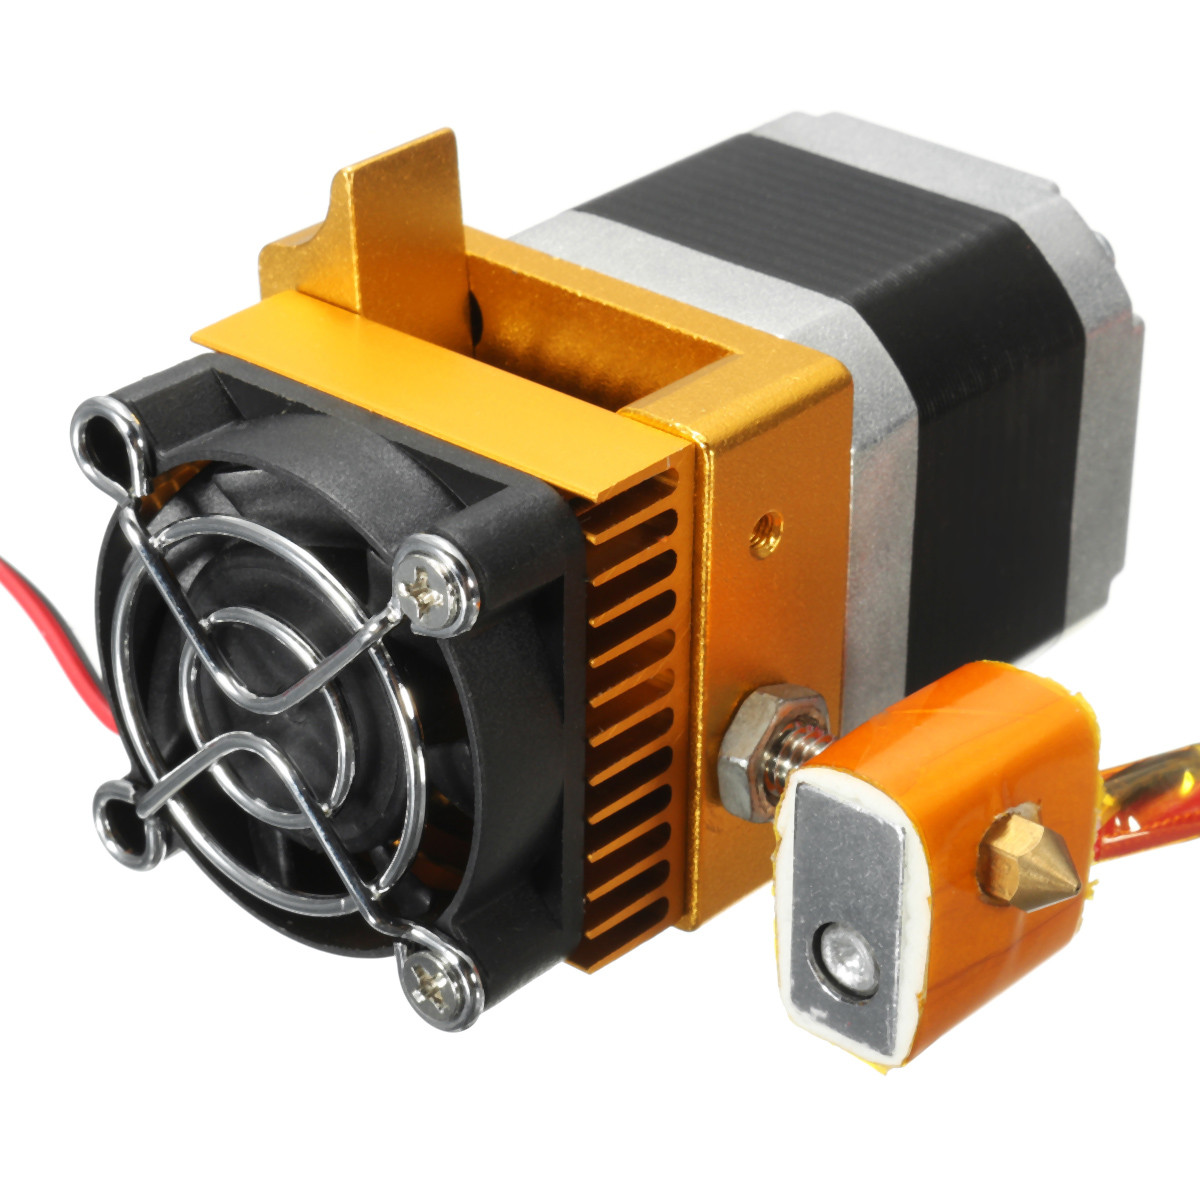
\includegraphics[width=\textwidth]{mk8-extruder}
        \caption{3D printer extruder}
        \label{fig:mk8-extruder}
    \end{subfigure}
    \begin{subfigure}[b]{0.4\textwidth}
        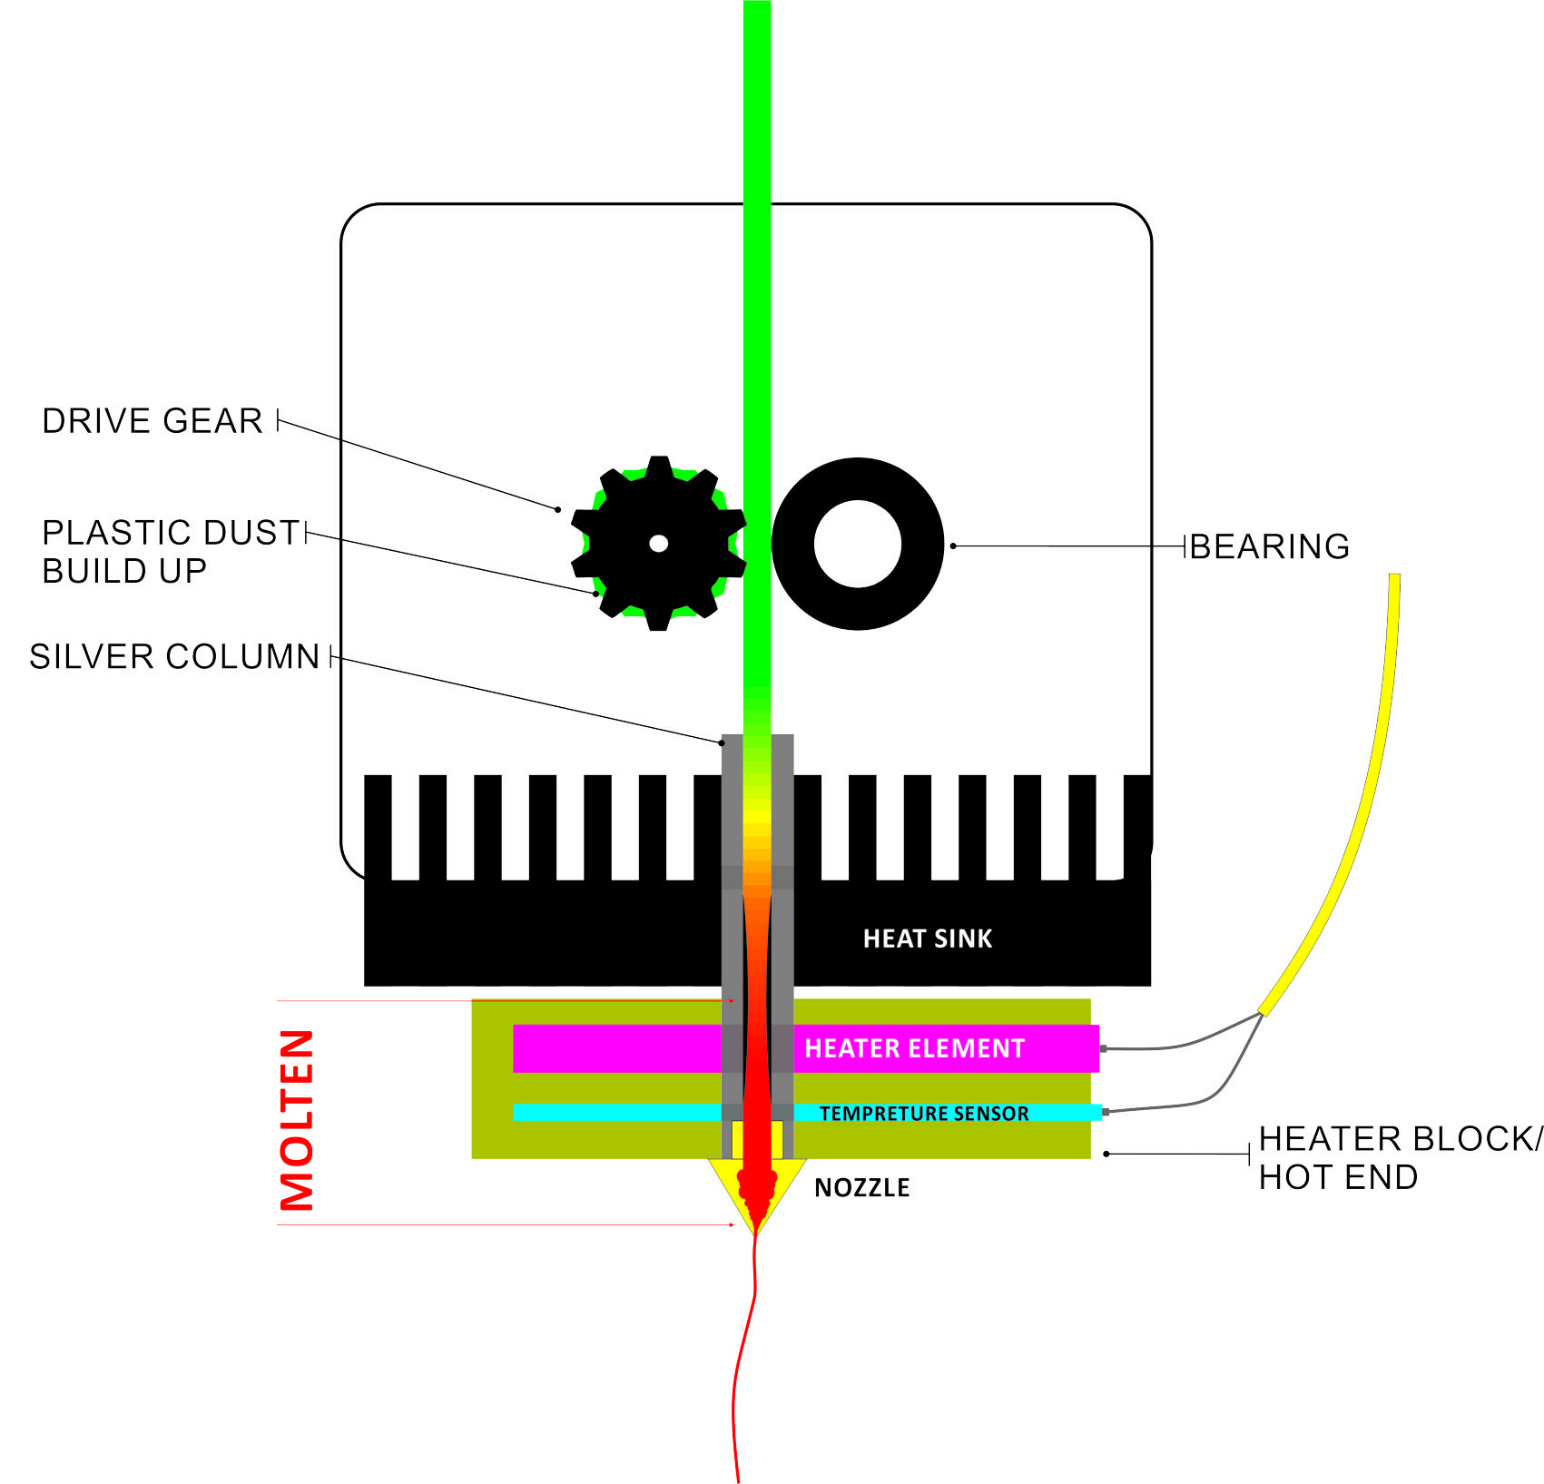
\includegraphics[width=\textwidth]{extruder-function}
        \caption{Functionality of extruder}
        \label{fig:extruder-function}
    \end{subfigure}
    \caption{3D printer extruder}
    \label{fig:extruder}
\end{figure}

\begin{figure}
    \centering
    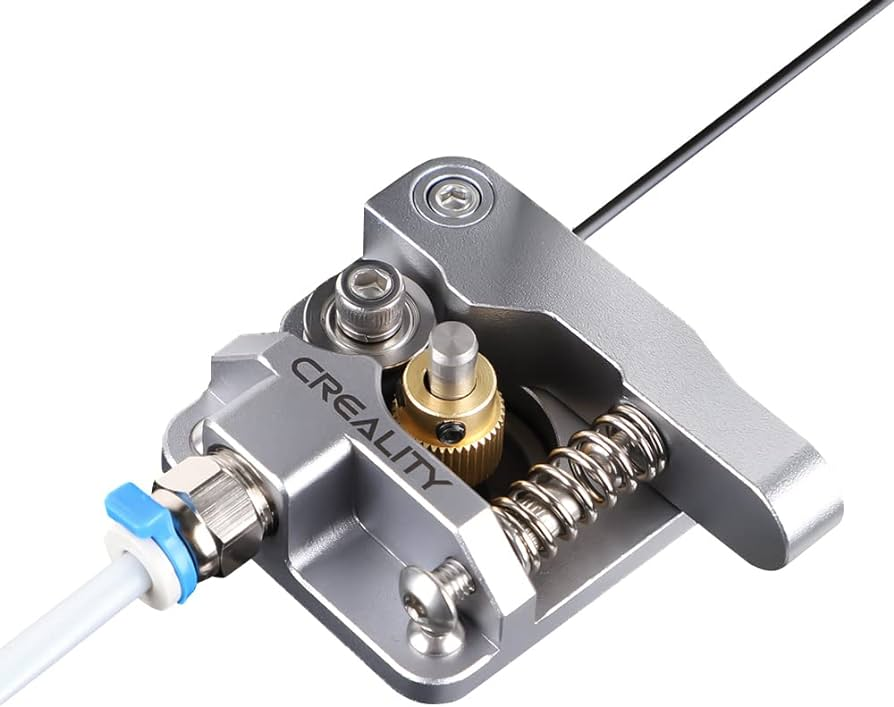
\includegraphics[width=0.5\textwidth]{creality-extruder}
    \caption{Extruder without heater}
    \label{fig:extruder-wo-heater}
\end{figure}


\begin{figure}
    \centering
    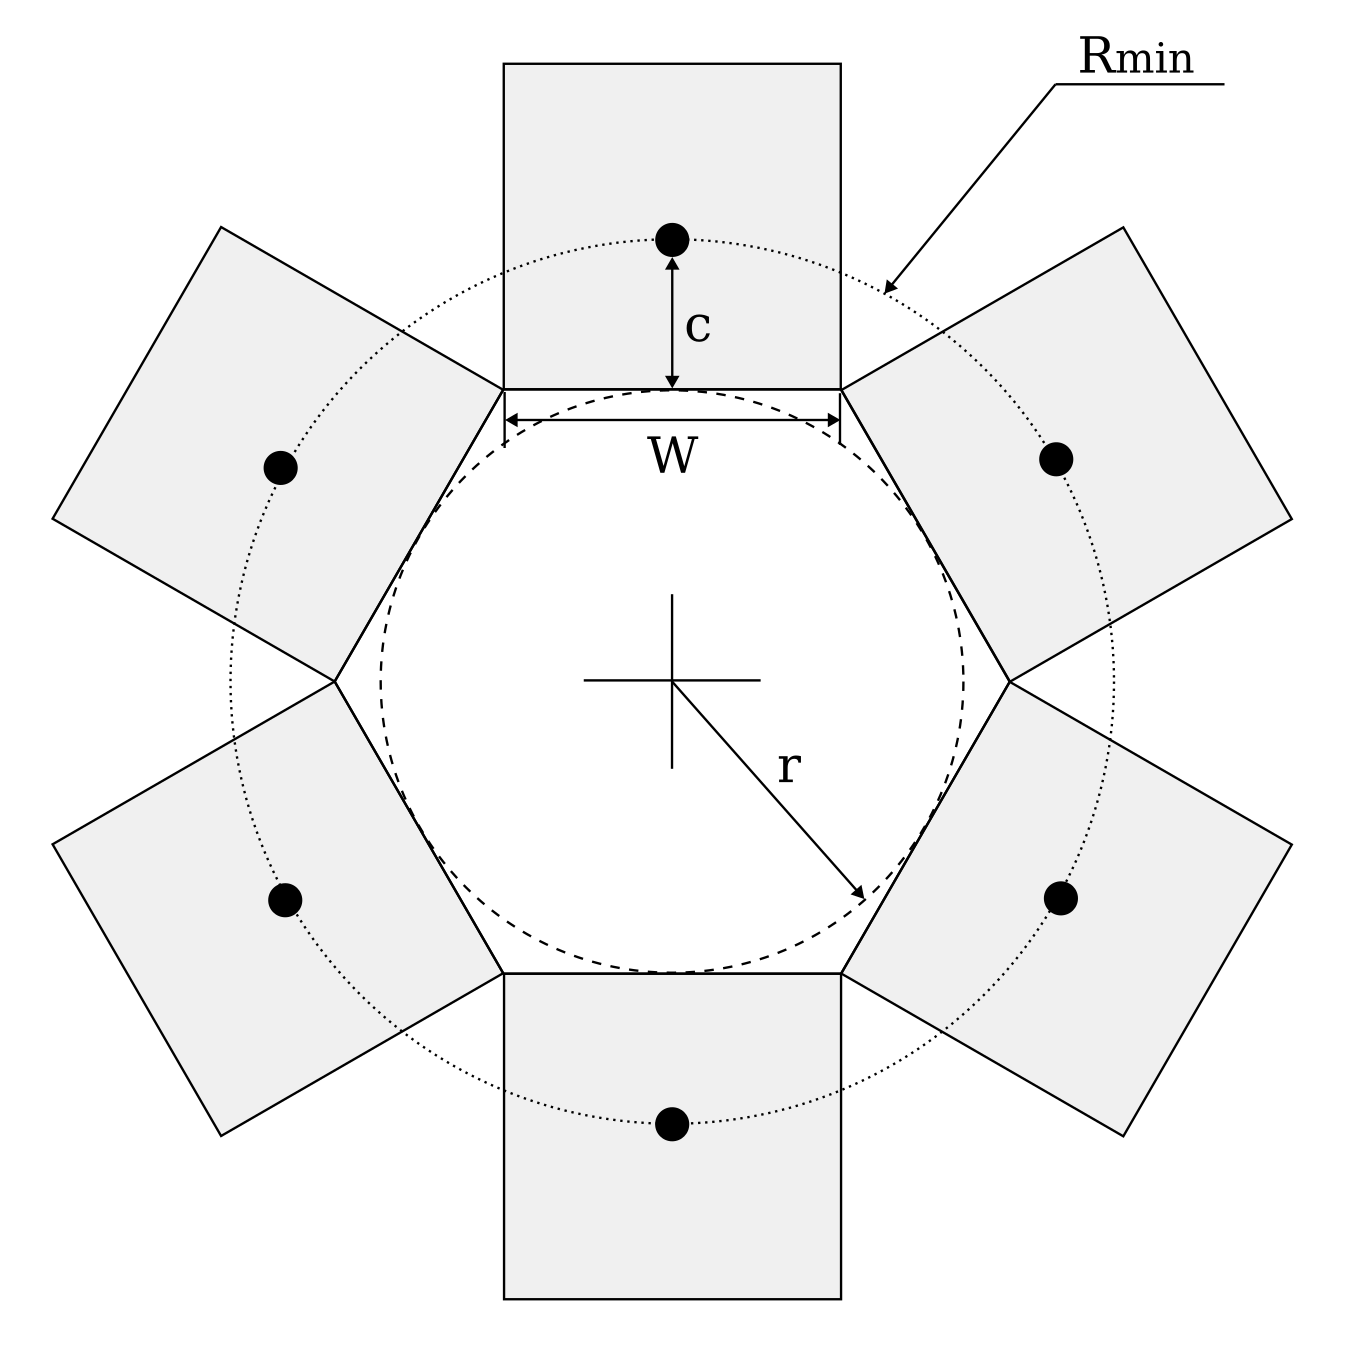
\includegraphics[width=0.7\textwidth]{actuators-arrange}
    \caption{Actuators arrange}
    \label{fig:actuators-arrange}
\end{figure}

$R_{min}=3.5$ cm, $c=0.5$ cm, $W\approx3.5$ cm

Original extruder $W=5.2$ cm, $c=0.7$ cm, $R_{min}=5.2$ cm

\begin{equation}
    r=R_{min}-c
\end{equation}

\begin{equation}
    W=\frac{2}{\sqrt{3}}r
\end{equation}

\begin{equation}
    W=\frac{2}{\sqrt{3}}(R_{min}-c)
\end{equation}

\begin{equation}
    R_{min}=\frac{\sqrt{3}}{2}W+c
\end{equation}


\section{Motor}

\begin{figure}
    \centering
    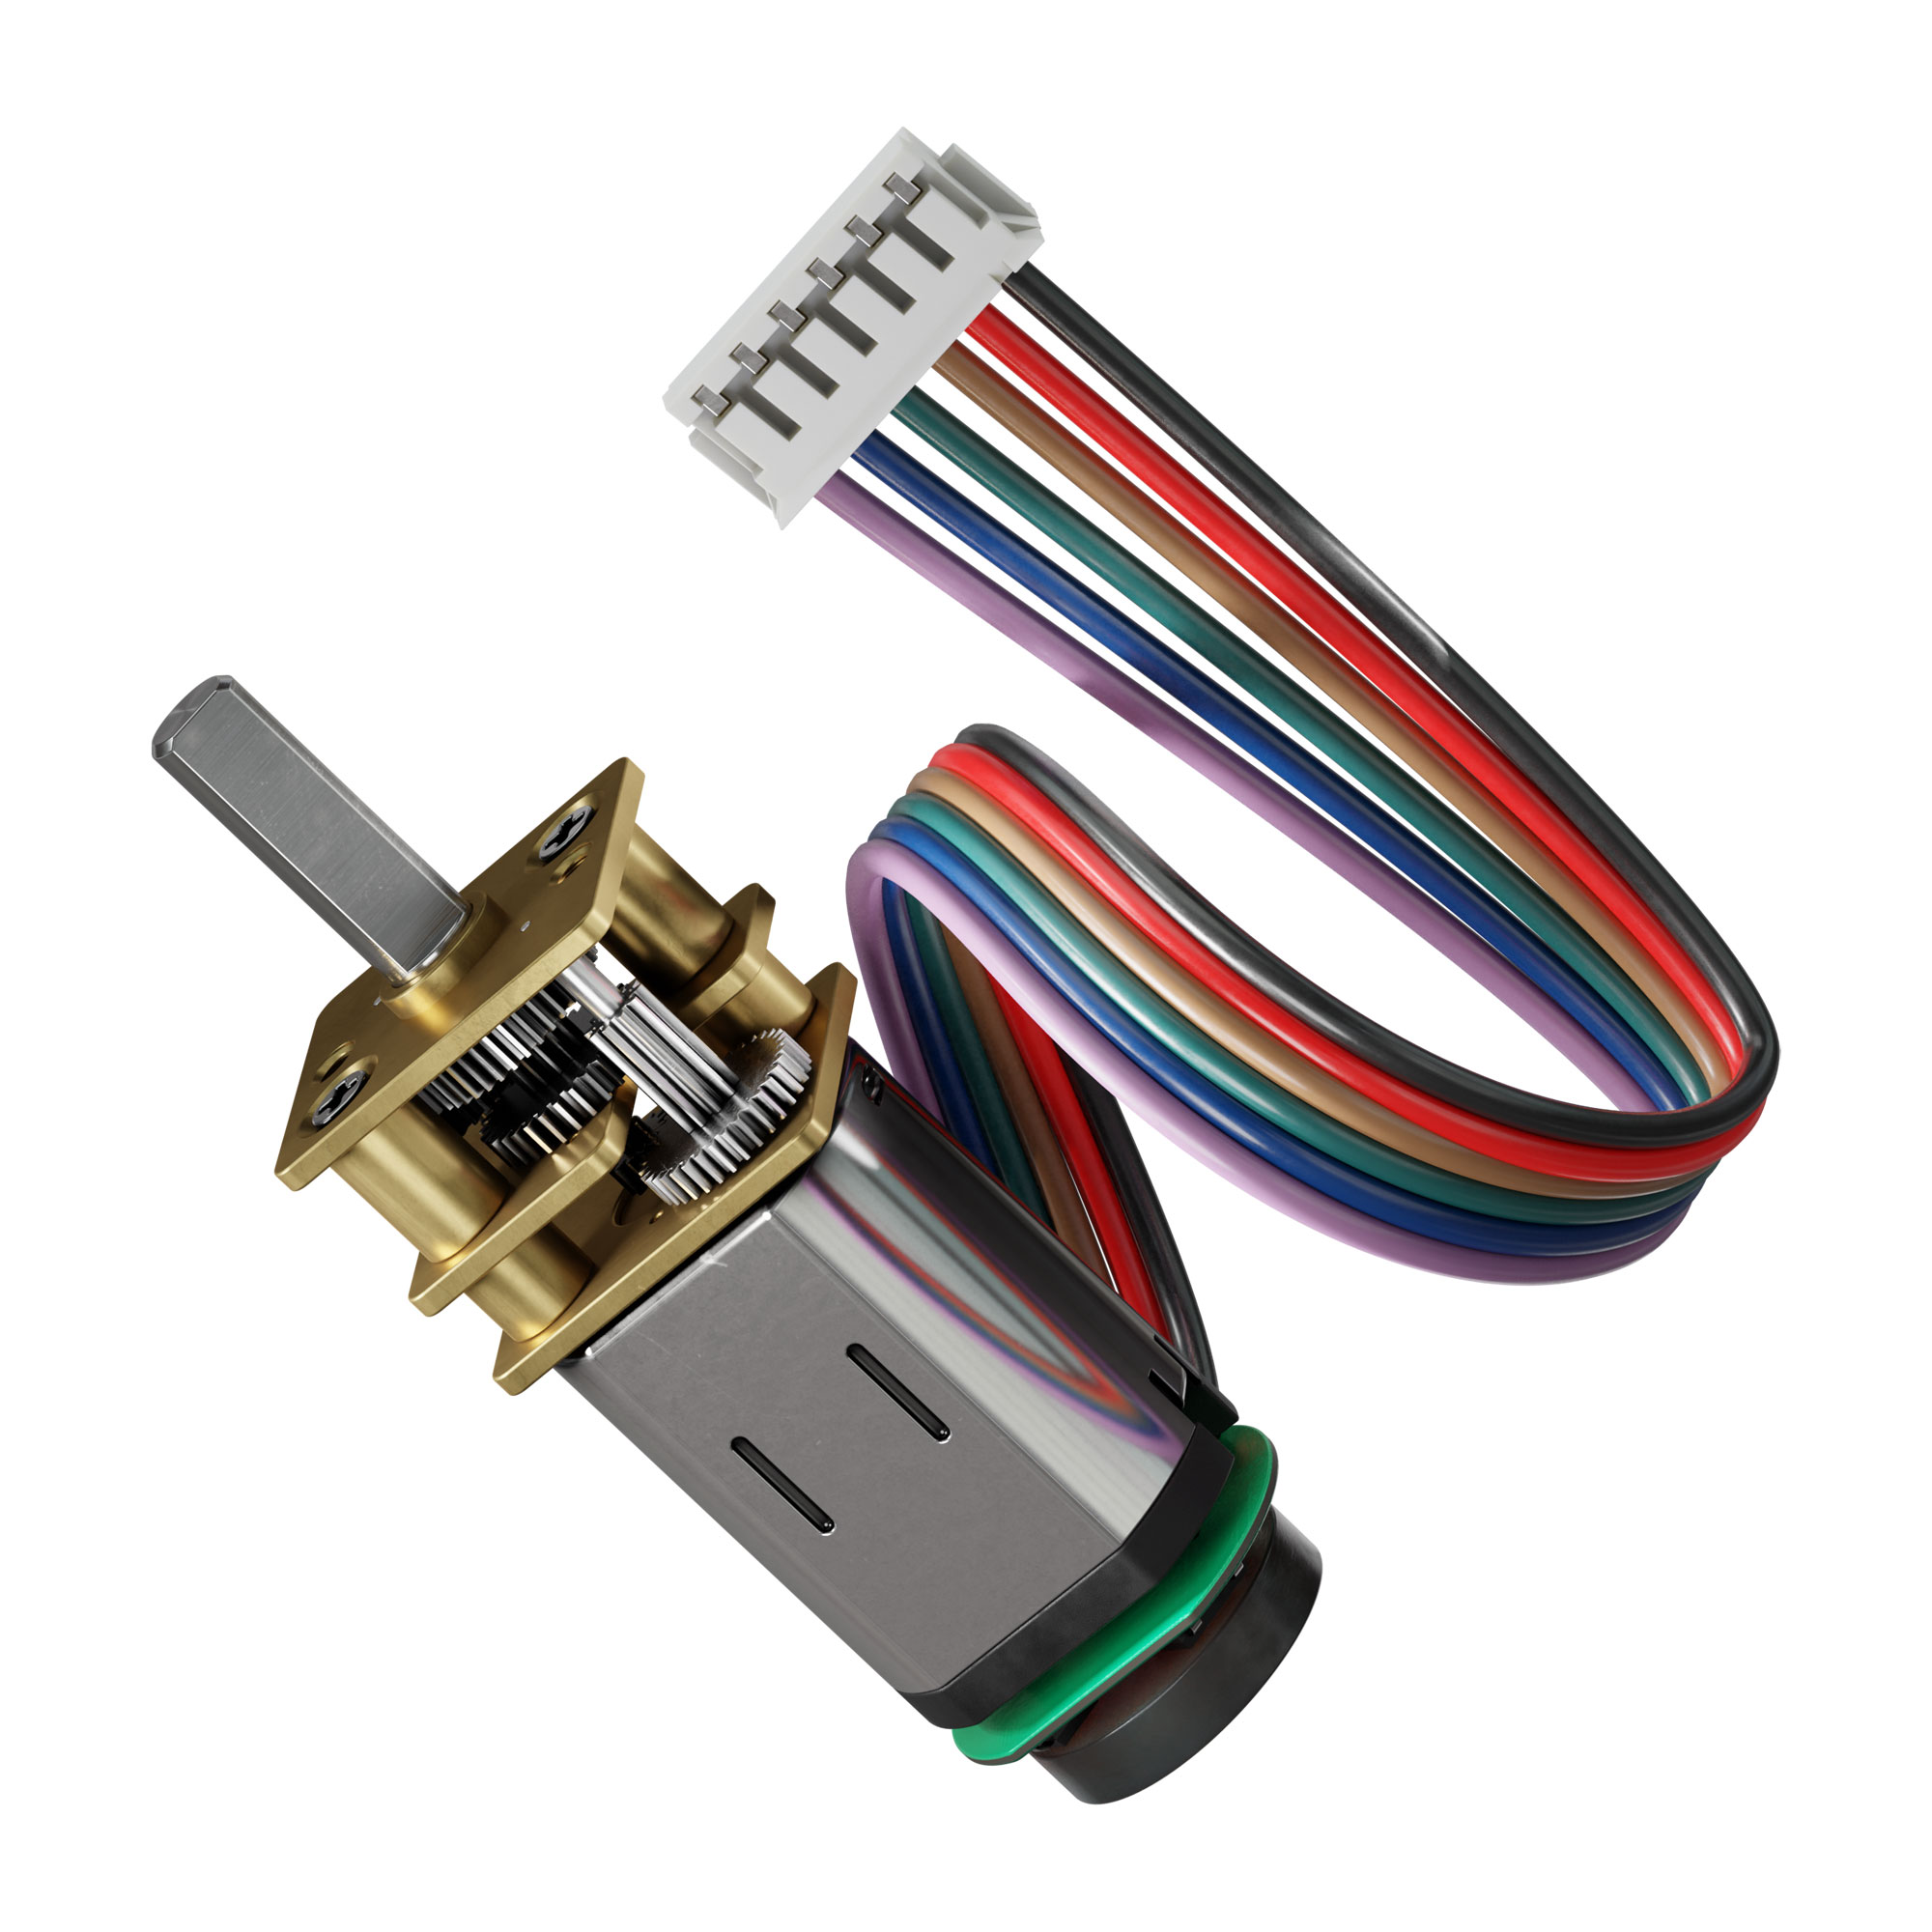
\includegraphics[width=0.45\textwidth]{n20-encoder}
    \caption{Gear motor N20 with encoder}
    \label{fig:n20-encoder}
\end{figure}

\begin{figure}
    \centering
    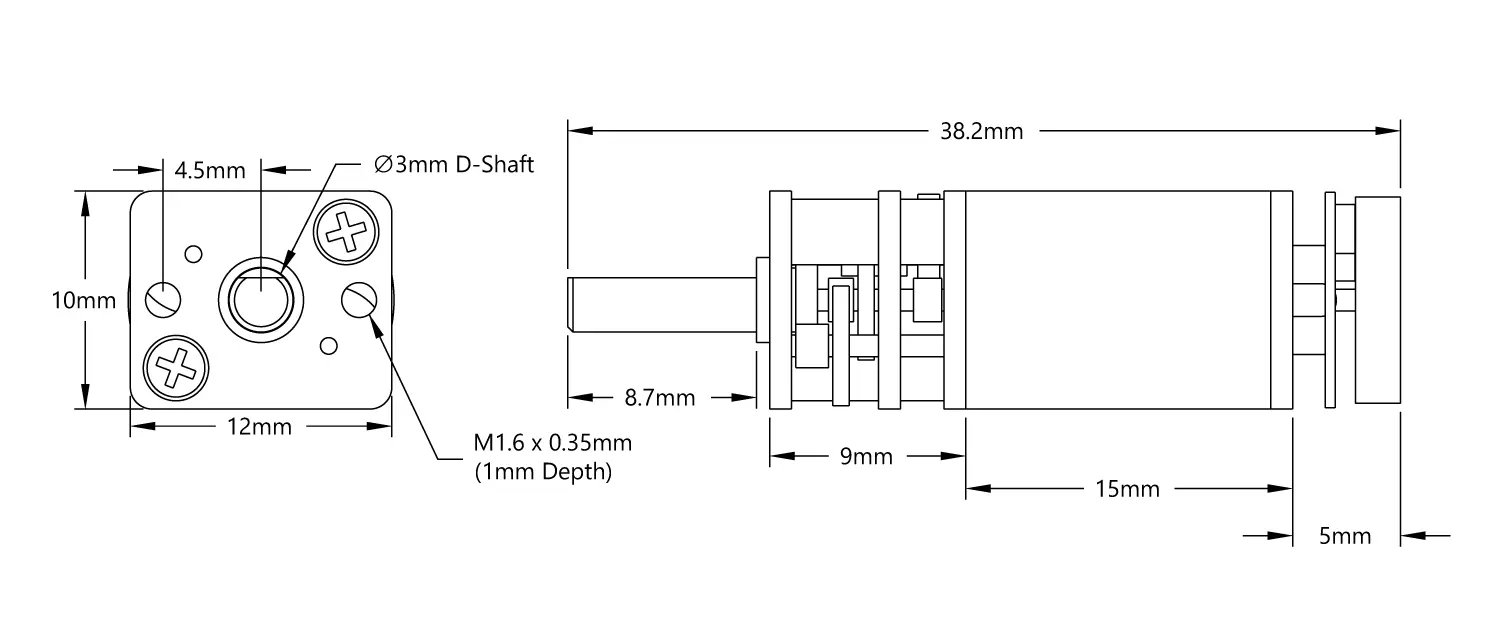
\includegraphics[width=0.9\textwidth]{n20-encoder-dimensions}
    \caption{Dimensions of gear motor N20 with encoder}
    \label{fig:n20-encoder-dimensions}
\end{figure}


\begin{table}[]
    \centering
    \caption{Gear motor specifications}
    \label{tab:motor-specs}
    \begin{tabular}{@{}ll@{}}
    \toprule
    Property                                     & Value                  \\
    \midrule
    Output shaft style                           & D-Shaft                \\
    Voltage range                                & $6-12$V                \\
    Speed (no load @ 6VDC)                       & $70$ rpm               \\
    Rated torque                                 & $0.65$ kg$\cdot$cm            \\
    Stall torque                                 & $4$ kg$\cdot$cm               \\
    Gear ratio                                   & 210:1                  \\
    Weight                                       & $15$g                  \\
    Encoder: cycles per revolution (motor shaft) & 3                      \\
    Encoder sensor type                          & Magnetic (Hall Effect) \\
    Hall response frequency                      & $100$ kHz              \\
    \bottomrule
    \end{tabular}
\end{table}

\section{First model}

\begin{figure}
    \centering
    \begin{subfigure}[b]{0.4\textwidth}
        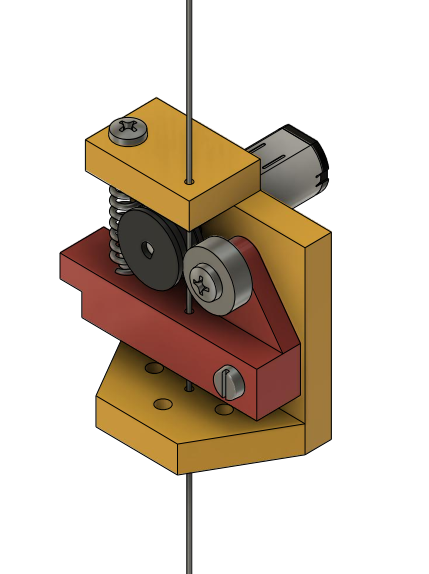
\includegraphics[width=\textwidth]{first-isometric-view-frontal}
        \caption{Front isometric view}
        \label{fig:first-front-isometric-view}
    \end{subfigure}
    \begin{subfigure}[b]{0.4\textwidth}
        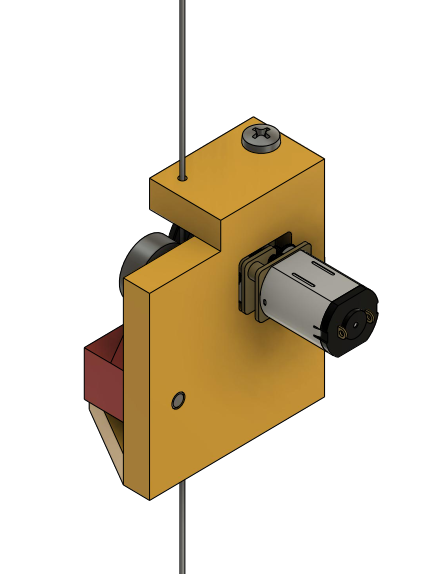
\includegraphics[width=\textwidth]{first-isometric-view-backwards}
        \caption{Back isometric view}
        \label{fig:first-back-isometric-view}
    \end{subfigure}
    \caption{First model isometric view}
    \label{fig:first-isometric-view}
\end{figure}

\begin{figure}
    \centering
    \begin{subfigure}[b]{0.272\textwidth}
        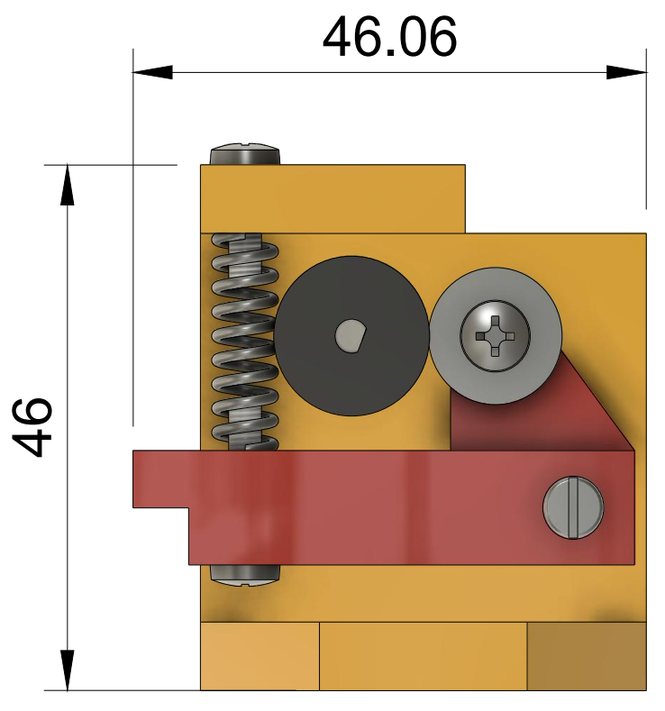
\includegraphics[width=\textwidth]{first-model-frontal}
        \caption{Front view}
        \label{fig:first-model-frontal}
    \end{subfigure}
    \begin{subfigure}[b]{0.628\textwidth}
        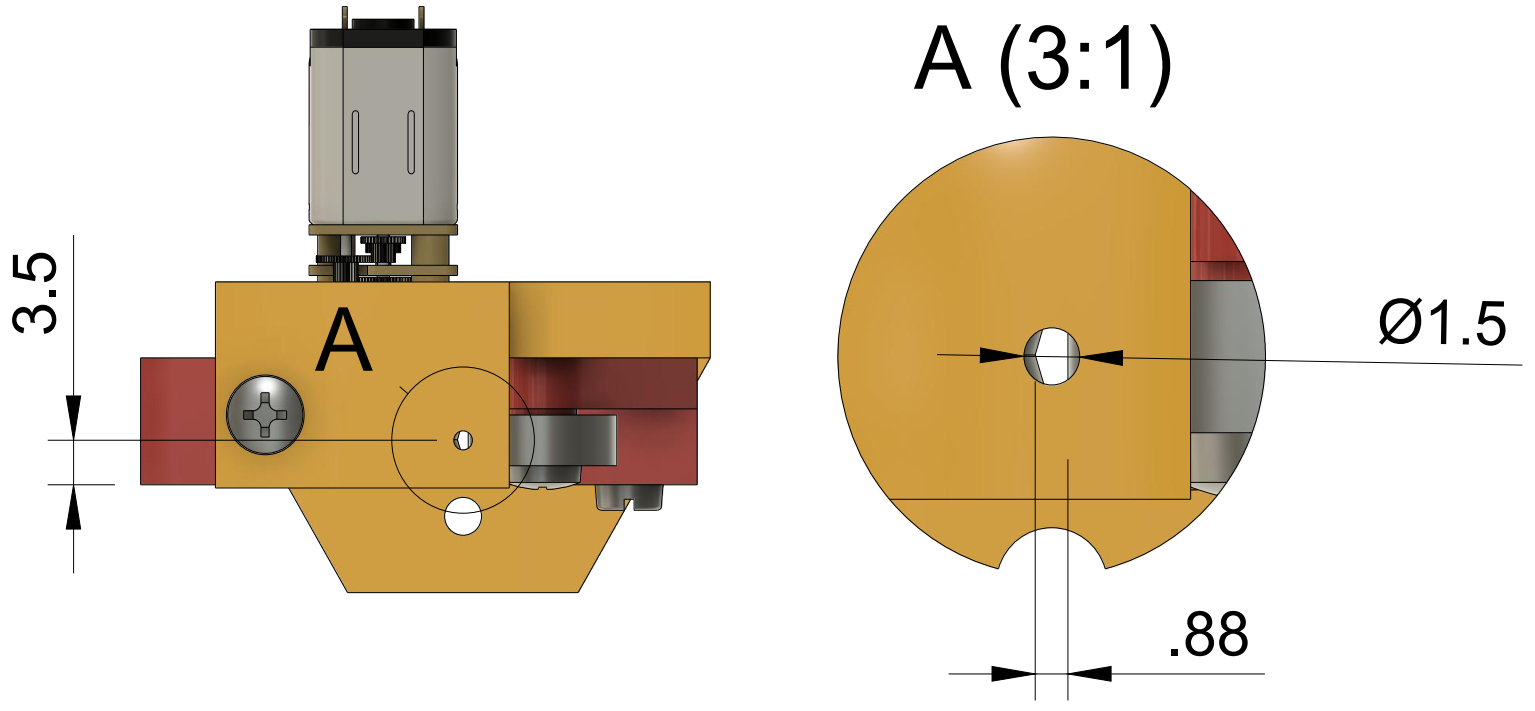
\includegraphics[width=\textwidth]{first-model-top-view}
        \caption{Top view}
        \label{fig:first-model-top-view}
    \end{subfigure}
    \caption{First model dimensions}
    \label{fig:first-model-dimensions}
\end{figure}

\section{Final model}

\begin{figure}
    \centering
    \begin{subfigure}[b]{0.4\textwidth}
        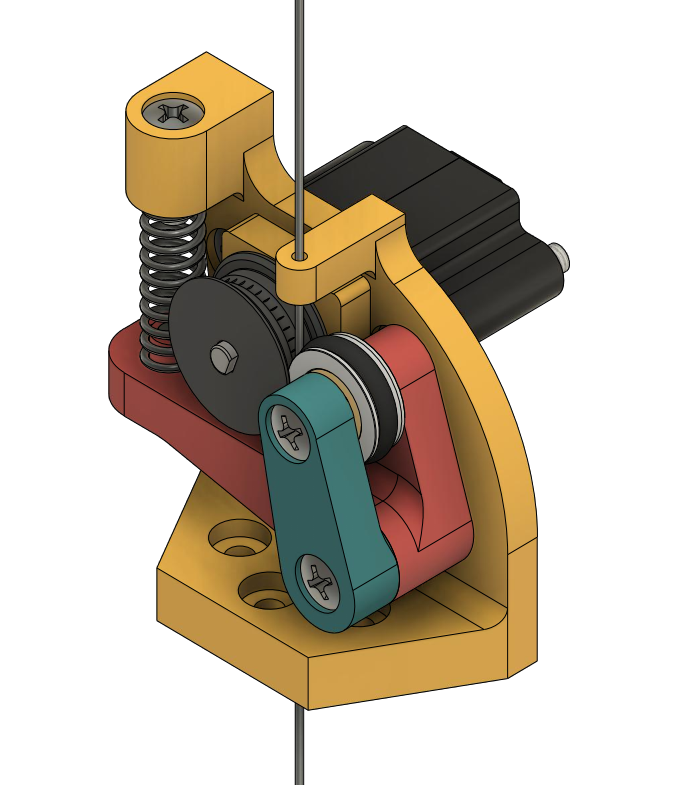
\includegraphics[width=\textwidth]{final-isometric-view-front}
        \caption{Front isometric view}
        \label{fig:final-front-isometric-view}
    \end{subfigure}
    \begin{subfigure}[b]{0.4\textwidth}
        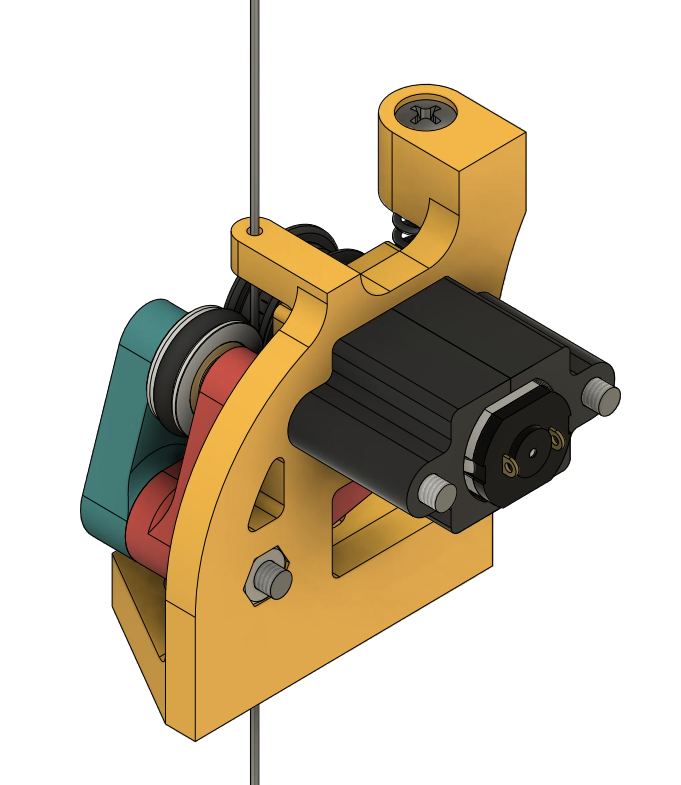
\includegraphics[width=\textwidth]{final-isometric-view-back}
        \caption{Back isometric view}
        \label{fig:final-back-isometric-view}
    \end{subfigure}
    \caption{Final model isometric view}
    \label{fig:final-isometric-view}
\end{figure}

\begin{figure}
    \centering
    \begin{subfigure}[b]{0.316\textwidth}
        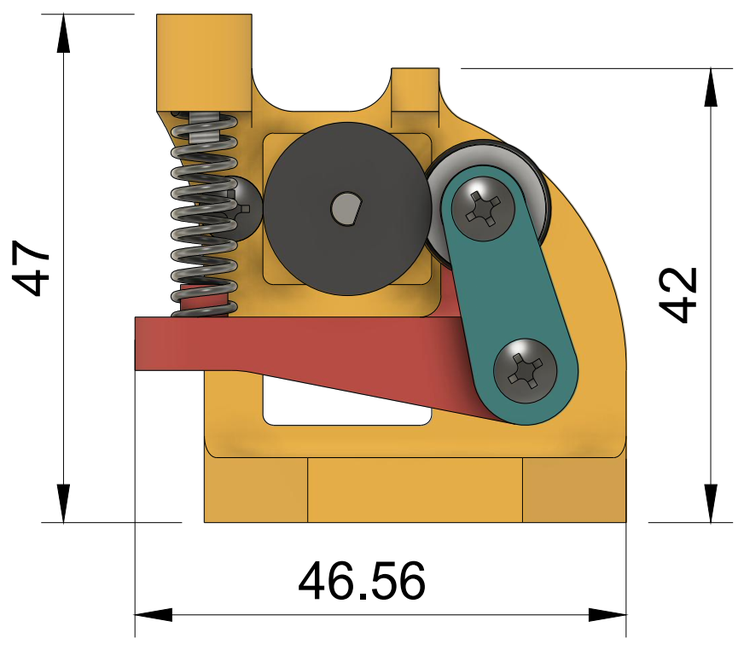
\includegraphics[width=\textwidth]{final-front}
        \caption{Front view}
        \label{fig:final-frontal}
    \end{subfigure}
    \begin{subfigure}[b]{0.584\textwidth}
        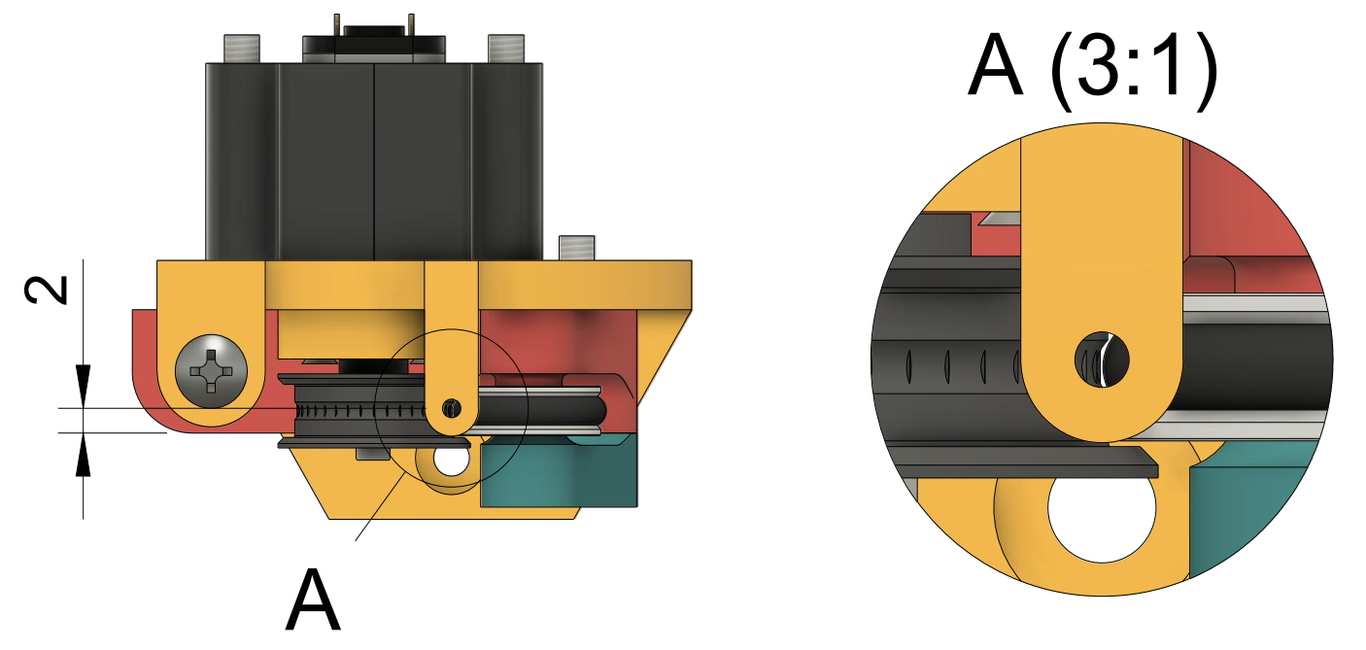
\includegraphics[width=\textwidth]{final-top}
        \caption{Top view}
        \label{fig:first-top}
    \end{subfigure}
    \caption{Final model dimensions}
    \label{fig:final-model-dimensions}
\end{figure}

\begin{figure}
    \centering
    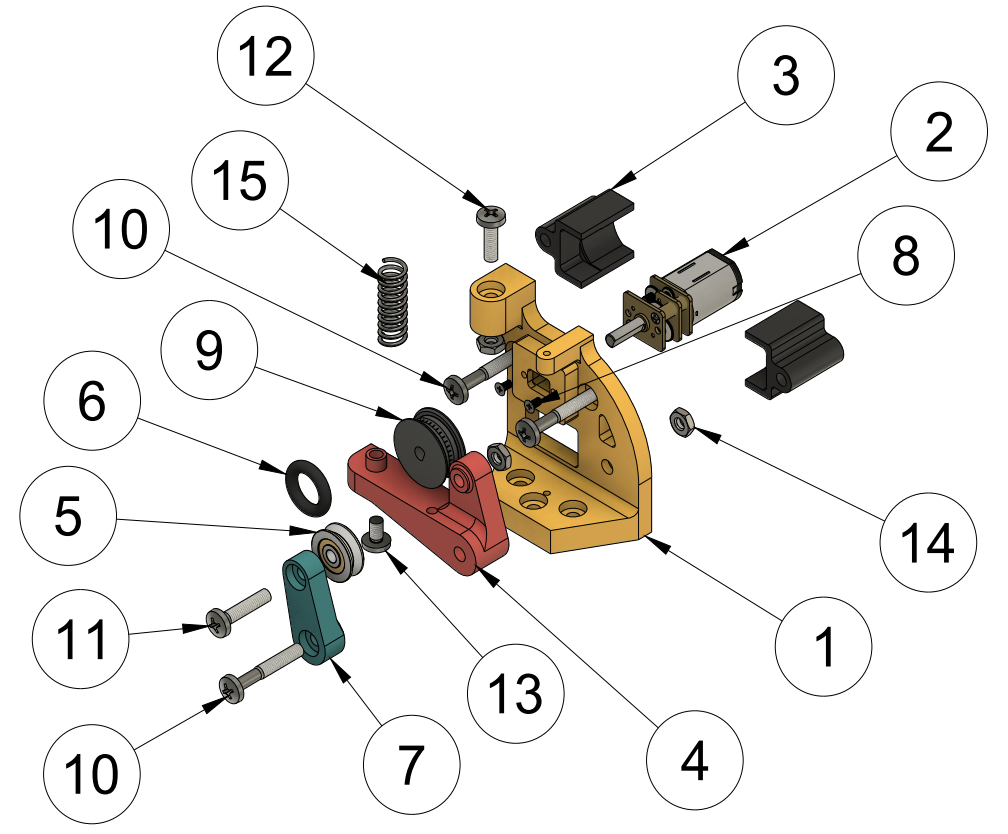
\includegraphics[width=0.8\textwidth]{actuator-final-explode}
    \caption{Actuator assembly exploded-view}
    \label{fig:final-actuator-explode}
\end{figure}
\begin{table}[h]
    \centering
    \caption{Actuator assembly parts list}
    \label{tab:final-actuator-parts}
    \begin{tabular}{llll}
    \toprule
    Item & Qty & Part Name / Description & Source \\
    \midrule
    1 & 1 & Base & 3D Printed \\
    2 & 1 & Motor GA12 N20 (must be with encoder) & Commercial \\
    3 & 2 & Motor Support & 3D Printed \\
    4 & 1 & Arm & 3D printed \\
    5 & 1 & V623ZZ Groove Pulley & Commercial \\
    6 & 1 & O-Ring - W2.62 x DI7.59 x DE2.83 & Commercial \\
    7 & 1 & Arm Support & 3D Printed \\
    8 & 2 & Phillips Countersunk Screw - DIN 965H M1.6x3 & Commercial \\
    9 & 1 & Pulley & 3D Printed \\
    10 & 3 & Binding Head Screw JIS B 1111 - M3x20 & Commercial \\
    11 & 1 & Binding Head Screw JIS B 1111 - M3x14 & Commercial \\
    12 & 1 & Binding Head Screw JIS B 1111 - M3x10 & Commercial \\
    13 & 1 & Binding Head Screw JIS B 1111 - M3x5 & Commercial \\
    14 & 3 & Hexagon Thin Nut DIN 439-2 - M3x0.5 & Commercial \\
    15 & 1 & Spring - D5.5x20mm & Manufactured \\
    \bottomrule
    \end{tabular}
\end{table}


\section{Specifications}

\begin{figure}
    \centering
    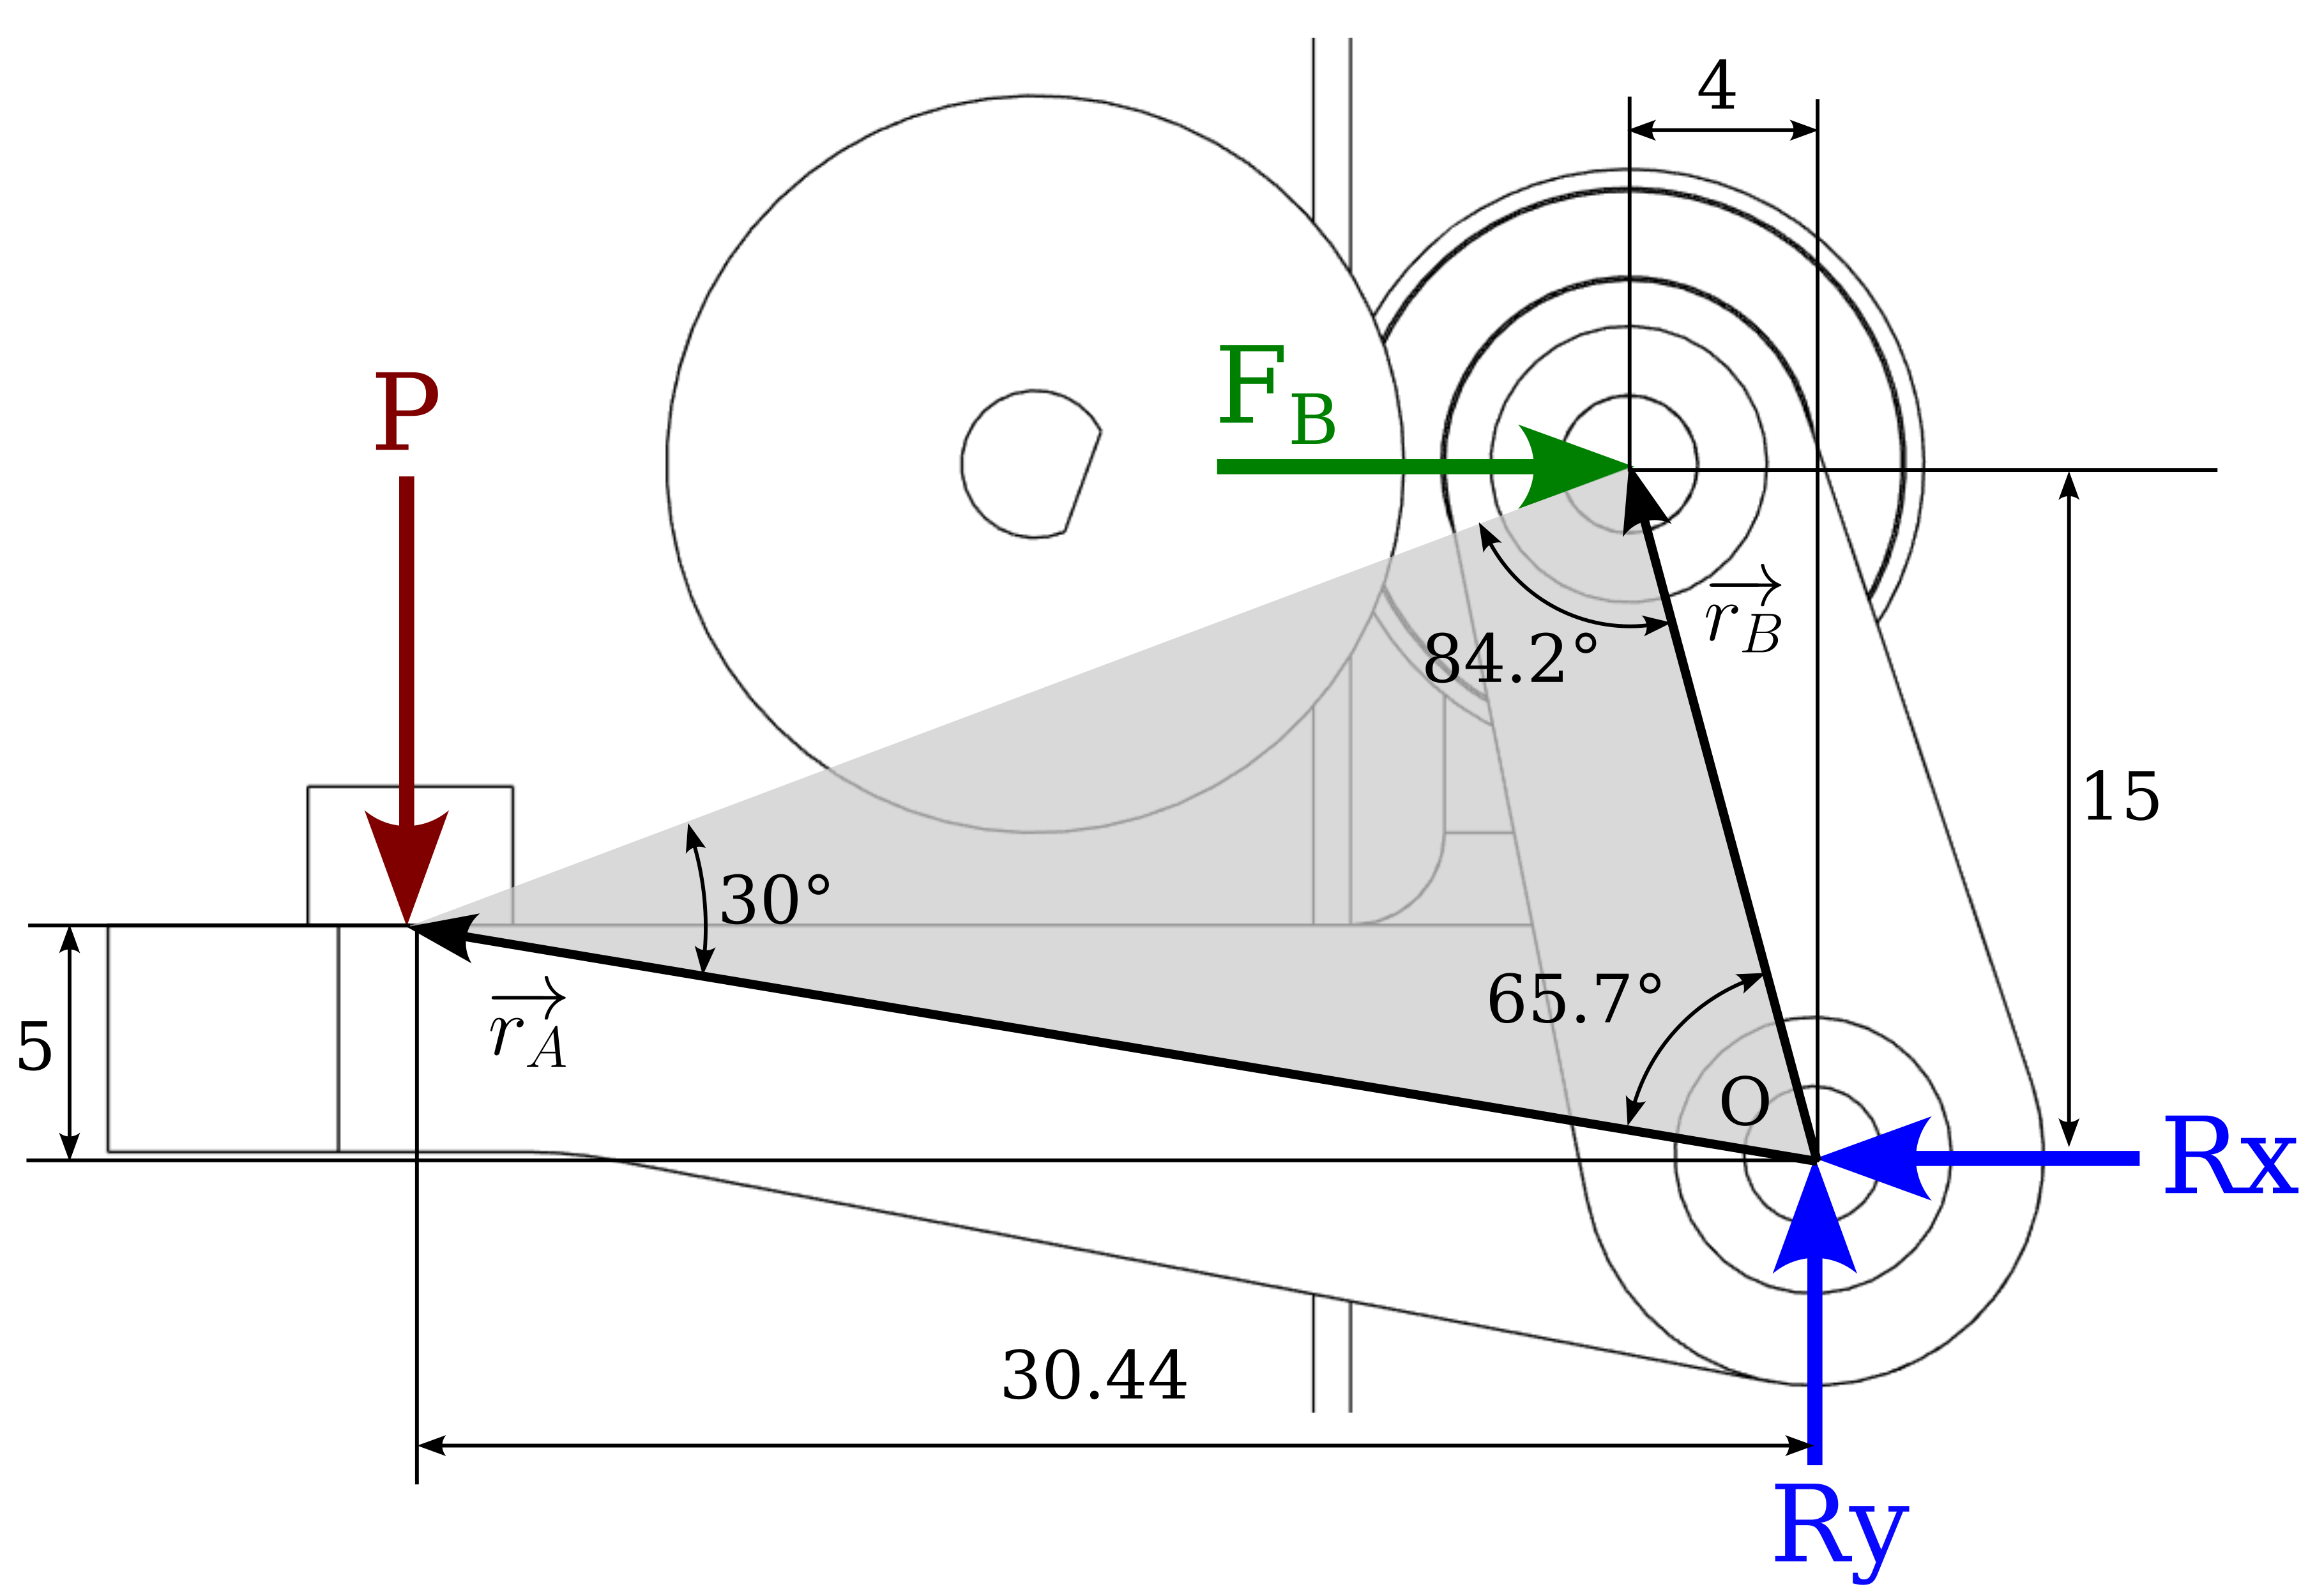
\includegraphics[width=0.8\textwidth]{forces-arm}
    \caption{Forces in actuator arm}
    \label{fig:forces-arm}
\end{figure}


\begin{align}
    \label{eq:sum-forces}
    \sum \myvec{F}=0 \quad\therefore& \quad \myvec{P} + \myvec{R_y} + \myvec{F_B}+\myvec{R_x} = 0 \\
    \label{eq:sum-momentums}
    \sum \myvec{M_O}=0 \quad\therefore& \quad \myvec{r_A}\times\myvec{P} + \myvec{r_B}\times\myvec{F_B} = 0
\end{align}
\begin{equation}
    \label{eq:force-p}
    P=-k\Delta y
\end{equation}
\begin{equation}
    \label{eq:force-fb}
    F_B = \frac{r_{A,x}}{r_{B,y}}P = \frac{30.44}{15}P=-2.0293k\Delta y
\end{equation}

\begin{figure}
    \centering
    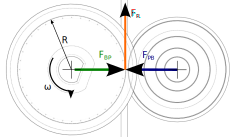
\includegraphics[width=0.7\textwidth]{friction-force}
    \caption{Friction force in rod}
    \label{fig:friction-force}
\end{figure}
\begin{equation}
    \label{eq:force-fbp}
    F_{BP}=F_B
\end{equation}
\begin{equation}
    \label{eq:force-fr}
    F_{R}=\mu_{s}F_{BP}=-2.0293\mu_{s}k\Delta y
\end{equation}

\begin{table}[h]
    \centering
    \caption{Actuator specification}
    \label{tab:actuator-specs}
    \begin{tabular}{ll}
    \toprule
    Property & Value \\
    \midrule
    Pulley ratio ($R$) & $5.3$ mm \\
    Maximum angular velocity ($\omega_{max}$) & $7.3304$ rad/s \\
    Maximum linear velocity ($v_{max}$) & $38.85$ mm/s \\
    \bottomrule
    \end{tabular}
\end{table}